% This is "sig-alternate.tex" V2.1 April 2013
% This file should be compiled with V2.5 of "sig-alternate.cls" May 2012
%
% This example file demonstrates the use of the 'sig-alternate.cls'
% V2.5 LaTeX2e document class file. It is for those submitting
% articles to ACM Conference Proceedings WHO DO NOT WISH TO
% STRICTLY ADHERE TO THE SIGS (PUBS-BOARD-ENDORSED) STYLE.
% The 'sig-alternate.cls' file will produce a similar-looking,
% albeit, 'tighter' paper resulting in, invariably, fewer pages.
%
% ----------------------------------------------------------------------------------------------------------------
% This .tex file (and associated .cls V2.5) produces:
%       1) The Permission Statement
%       2) The Conference (location) Info information
%       3) The Copyright Line with ACM data
%       4) NO page numbers
%
% as against the acm_proc_article-sp.cls file which
% DOES NOT produce 1) thru' 3) above.
%
% Using 'sig-alternate.cls' you have control, however, from within
% the source .tex file, over both the CopyrightYear
% (defaulted to 200X) and the ACM Copyright Data
% (defaulted to X-XXXXX-XX-X/XX/XX).
% e.g.
% \CopyrightYear{2007} will cause 2007 to appear in the copyright line.
% \crdata{0-12345-67-8/90/12} will cause 0-12345-67-8/90/12 to appear in the copyright line.
%
% ---------------------------------------------------------------------------------------------------------------
% This .tex source is an example which *does* use
% the .bib file (from which the .bbl file % is produced).
% REMEMBER HOWEVER: After having produced the .bbl file,
% and prior to final submission, you *NEED* to 'insert'
% your .bbl file into your source .tex file so as to provide
% ONE 'self-contained' source file.
%
% ================= IF YOU HAVE QUESTIONS =======================
% Questions regarding the SIGS styles, SIGS policies and
% procedures, Conferences etc. should be sent to
% Adrienne Griscti (griscti@acm.org)
%
% Technical questions _only_ to
% Gerald Murray (murray@hq.acm.org)
% ===============================================================
%
% For tracking purposes - this is V2.0 - May 2012

\documentclass{sig-alternate-05-2015}
\usepackage{graphicx}
\graphicspath{ {} }


\begin{document}

% Copyright
\setcopyright{acmcopyright}
%\setcopyright{acmlicensed}
%\setcopyright{rightsretained}
%\setcopyright{usgov}
%\setcopyright{usgovmixed}
%\setcopyright{cagov}
%\setcopyright{cagovmixed}


% DOI
\doi{10.475/123_4}

% ISBN
\isbn{123-4567-24-567/08/06}

%Conference
%\conferenceinfo{PLDI '13}{June 16--19, 2013, Seattle, WA, USA}

%\acmPrice{\$0.00}

%
% --- Author Metadata here ---
\conferenceinfo{MSR}{2016 Austin, Texas USA}
%\CopyrightYear{2007} % Allows default copyright year (20XX) to be over-ridden - IF NEED BE.
%\crdata{0-12345-67-8/90/01}  % Allows default copyright data (0-89791-88-6/97/05) to be over-ridden - IF NEED BE.
% --- End of Author Metadata ---

\title{Most common replacements performed by programmers when fixing bugs}

%
% You need the command \numberofauthors to handle the 'placement
% and alignment' of the authors beneath the title.
%
% For aesthetic reasons, we recommend 'three authors at a time'
% i.e. three 'name/affiliation blocks' be placed beneath the title.
%
% NOTE: You are NOT restricted in how many 'rows' of
% "name/affiliations" may appear. We just ask that you restrict
% the number of 'columns' to three.
%
% Because of the available 'opening page real-estate'
% we ask you to refrain from putting more than six authors
% (two rows with three columns) beneath the article title.
% More than six makes the first-page appear very cluttered indeed.
%
% Use the \alignauthor commands to handle the names
% and affiliations for an 'aesthetic maximum' of six authors.
% Add names, affiliations, addresses for
% the seventh etc. author(s) as the argument for the
% \additionalauthors command.
% These 'additional authors' will be output/set for you
% without further effort on your part as the last section in
% the body of your article BEFORE References or any Appendices.

\numberofauthors{3} %  in this sample file, there are a *total*
% of EIGHT authors. SIX appear on the 'first-page' (for formatting
% reasons) and the remaining two appear in the \additionalauthors section.
%
\author{
% You can go ahead and credit any number of authors here,
% e.g. one 'row of three' or two rows (consisting of one row of three
% and a second row of one, two or three).
%
% The command \alignauthor (no curly braces needed) should
% precede each author name, affiliation/snail-mail address and
% e-mail address. Additionally, tag each line of
% affiliation/address with \affaddr, and tag the
% e-mail address with \email.
%
% 1st. author
\alignauthor
Mauricio Soto\\
       \affaddr{Carnegie Mellon University}\\
       \affaddr{Pittsburgh, PA}\\
       \email{mauriciosoto@cmu.edu}
% 2nd. author
\alignauthor Chu Pan Wong   
       \affaddr{Carnegie Mellon University}\\
       \affaddr{Pittsburgh, PA}\\
       \email{email@domain.com}       
\and  % use '\and' if you need 'another row' of author names
% 3rd. author
\alignauthor Ferdinand Lastname
       \affaddr{Carnegie Mellon University}\\
       \affaddr{Pittsburgh, PA}\\
       \email{email@domain.com}
% 4th. author
\alignauthor
Claire Le Goues\\
       \affaddr{Carnegie Mellon University}\\
       \affaddr{Pittsburgh, PA}\\
       \email{clegoues@cs.cmu.edu}
}
% There's nothing stopping you putting the seventh, eighth, etc.
% author on the opening page (as the 'third row') but we ask,
% for aesthetic reasons that you place these 'additional authors'
% in the \additional authors block, viz.
%\additionalauthors{Additional authors: John Smith (The Th{\o}rv{\"a}ld Group,
%email: {\texttt{jsmith@affiliation.org}}) and Julius P.~Kumquat
%(The Kumquat Consortium, email: {\texttt{jpkumquat@consortium.net}}).}
\date{February 2, 2016}
% Just remember to make sure that the TOTAL number of authors
% is the number that will appear on the first page PLUS the
% number that will appear in the \additionalauthors section.

\maketitle
\begin{abstract}
\textbf{
With the rise of automated program repair in the last couple of years, there are a lot of questions to remain unanswered. We performed a study on the Github dump of September 2015 in which we analyzed all the fixing revisions of this dataset, and found all the replacements made in these 46,301,429 files from real life projects in Github.
}

\textbf{
We found very valuable information to guide automatic software repair, such as the most common and least common replacements made by human developers in order to build a successful patch; we analyzed the most and least common statement to replace others, and the most and least likely statement to get replaced by other. We also analyzed, once you have a statement that you want to replace (a faulty statement), what are the most likely statements to replace it for. These information will help automatic program repair tools to be more maintainable and user friendly, taking it one step closer to what humans developers do to repair their code.
}

\end{abstract}


%
% The code below should be generated by the tool at
% http://dl.acm.org/ccs.cfm
% Please copy and paste the code instead of the example below. 
%
\begin{CCSXML}
<ccs2012>
 <concept>
  <concept_id>10010520.10010553.10010562</concept_id>
  <concept_desc>Computer systems organization~Embedded systems</concept_desc>
  <concept_significance>500</concept_significance>
 </concept>
 <concept>
  <concept_id>10010520.10010575.10010755</concept_id>
  <concept_desc>Computer systems organization~Redundancy</concept_desc>
  <concept_significance>300</concept_significance>
 </concept>
 <concept>
  <concept_id>10010520.10010553.10010554</concept_id>
  <concept_desc>Computer systems organization~Robotics</concept_desc>
  <concept_significance>100</concept_significance>
 </concept>
 <concept>
  <concept_id>10003033.10003083.10003095</concept_id>
  <concept_desc>Networks~Network reliability</concept_desc>
  <concept_significance>100</concept_significance>
 </concept>
</ccs2012>  
\end{CCSXML}


%
% End generated code
%

%
%  Use this command to print the description
%
\printccsdesc

% We no longer use \terms command
%\terms{Theory}

\keywords{Automatic error repair; Maintainability; Human-like patches}

\section{Introduction}
Automatic bug repair is the branch of computer science that deals with automated ways to repair errors in software. There have been several approaches taken towards improving the different methodologies to repair bugs in software automatically \cite{dongsun}\cite{weimer}\cite{claire} \cite{kai}, one of the most accepted approaches so far has been GenProg \cite{weimer}\cite{claire}, which is an evolutionary program repair tool and applies four different kinds of possible changes to code in order to find a patch for a given bug. These changes are the following: Delete, Replace, Swap and Append.

Our research aims to provide guidelines to improve three out of four of these possible changes: Delete, Replace and Append. It will provide the data necessary for this tool and other approaches to have a guide on what is the way in which human programmers change their code when coding a fix for a bug. This way it will make it more likely for automatic error repair approaches to succeed in finding a patch for a particular error, and also, to provide automatic error repair software with heuristics to make the patches more human-like and therefore more readable and maintainable by human developers.

In this article we study the frequency with which human programmers replace, delete and append different statements to their source code in order to fix a bug.


\section{Methodology}
Our methodology is applied to the latest official data dump of Github as of September 2015 provided by \cite{robert}.

\subsection{Statements}
Statements are the building blocks of software. There are several kinds of statements in which software can be divided into. In our approach we are trying to find patterns in the way human programmers replace, delete or append statements in order to fix a bug in their code.

The definitions of statements vary slightly depending on the programming language being used, but regardless of this, the vast majority of statements classifications are very similar independent of the language used. For our study we took a very standard classification of statements provided by the Java Development Tools package.

In this classification we have twenty two kinds of statements, from which we took fifteen of them for the gathering and analysis of our data. The list of statements taken for our analysis is the following:

\begin{verbatim}
AssertStatement
BreakStatement
ContinueStatement 
DoStatement 
ForStatement 
IfStatement 
LabeledStatement
ReturnStatement 
SwitchCase 
SwitchStatement 
SynchronizedStatement
ThrowStatement 
TryStatement 
TypeDeclarationStatement
WhileStatement
\end{verbatim}

The remaining six kinds of statements were not considered to be part of our analysis for three main reasons. We will start with this following statement type:

\begin{verbatim}
Block
\end{verbatim}

The statement type known as "Block" was not included since our main goal is to provide guidelines to automatic bug repair software to be able to create patches in a more guided way. It is irrelevant for an automatic bug repair software to know that an statement was replaced by a "Block", since a Block is an unknown amount of statements concatenated together and knowing that there is an infinite amount of possible permutations of statements that can be a Block, makes it useless to know that an statement was replaced by a Block, since a Block can be basically any possible combination of statements.

The next statement type:
\begin{verbatim}
EmptyStatement 
\end{verbatim}

The statement known as "EmptyStatement" is an statement that doesn't perform any action. Therefore, replacing any statement for an empty statement is equivalent to deleting that statement, and that case is treated separately.

The third reason of why the remaining five statement types were not included in the analysis is because these statement types are not supported by Boa as a StatementKind to the best of our knowledge. The remaining five statement types are the following:

\begin{verbatim}
ConstructorInvocation
EnhancedForStatement
ExpressionStatement
SuperConstructorInvocation
VariableDeclarationStatement
\end{verbatim}

We focused on the initial list of fifteen statement kinds mentioned at the beginning of the section.

\begin{table*}
\centering
\caption{Amount of appearances per replace kind}
\resizebox{\textwidth}{100pt}{
\begin{tabular}{|l|c|c|c|c|c|c|c|c|c|c|c|c|c|c|c|} \hline
 &Assert&Break&Continue&Do& For&If&Label&Return&Switch&Switch& Synchronized&Throw&Try&TypeDecl&While
\\ \hline
\texttt{Assert}	&-&340&	232	&27	&517	&1764&	14&	1260	&211	&191&	82&	1004	&352	&0	&206
\\ \hline
\texttt{Break} &455	&-&	1254&	176	&3757	&9096&	90&	10538&	771	&455&	672	&3123&	3660&	18&	2278
 \\ \hline
\texttt{Continue} & 229	&1384	&-&	221	&1909	&3094&	85&	3486	&772&	635	&233&	1227&	1493&	30&	1086
 \\   \hline
\texttt{Do} &32	&205&	171	&-&	474	&648	&12&	543	&106	&92&	44	&227	&325&	4&	558
  \\ \hline
\texttt{For} &505	&3366	&1516	&316	&-&	14547	&56	&14924	&2791	&1852	&1044&	5642&	5796	&41	&6582
 \\ \hline
\texttt{If}& 1402&	8820&	2430&	476	&13703&-&		247	&30489	&8639	&5710	&2472&	8960&	13714&	84&	5622
 \\ \hline
\texttt{Label} &19&	44	&46	&6&	56	&255	&-&	270	&44	&22	&5	&80&	53&	2	&33
\\ \hline
\texttt{Return} &1219&	8603	&3009	&531	&12620	&28536&	164	&-&	6088&	3657&	2021&	15346&	11486&	71	&4684
 \\ \hline
\texttt{Case} &298	&839&	506	&125&	3002&	8039&	33&	6261	&-&	126	&649&	2206&	2784&	24&	1864
\\ \hline
\texttt{Switch}&281	&533&	379	&56	&1997	&5175&	22	&4090&	126	&-&	212	&1571	&1311	&7&	878
 \\ \hline
\texttt{Synchronized} &79&	606&	289&	66	&1122&	3070&	158&	2853	&562&	256	&-&	1303&	1274&	8	&466
 \\ \hline
\texttt{Throw} &821&	2844&	1195	&197&	5993	&10664&	113&	16688&	2002	&1446&	936		&-&4443&	37&	1934
 \\ \hline
\texttt{Try}& 440&	3976&	1254&	214	&6414&	16294&	45	&14119	&3178	&1509	&1243&	4795	&-&	46&	2218
 \\ \hline
\texttt{TypeDecl} &2&	35&	15	&1&	49	&83&	1&	137	&21&	9&	4&	35&	46	&-&	11
 \\ \hline
\texttt{While}& 301&	2295&	1016&	937	&8257&	6587&	41	&6280&	1866&	766	&606&	2028&	2677&	27	&-
 \\ \hline
\end{tabular}
}
\end{table*}


\subsection{Data Collection}
We used the Boa platform \cite{robert} to be able to query the Github repository looking for patterns that humans use to patch errors in the their code. Our main goal is to provide automatic error fixing approaches with the data necessary to be able to replace, delete and append statements in the patches being created by them.
 
Our Boa queries are divided in two types:

\subsubsection{Replace Query}
The replace query is a query in which first we set the project that we are going to use, which is the Github dump of September 2015 provided by \cite{robert}. 

We then create a visitor to traverse all the nodes of this repository. First thing the visitor does is to ask weather the node is a Revision, and if it is, then it asks if it is a fixing revision. Therefore we are analyzing only files that were already committed and are now being reviewed to fix an error. We use Boa's infrastructure to do this by visiting the node they label as "Revision" and then calling the function defined by Boa "isfixingrevision()".

A replacement needs two statements, one that is deleted and another one that is inserted.
We then go through all the files that have been changed in this data set asking for two conditions: it must be a fixing revision and there must have been a previous version of this file before. If these conditions are met then we initialize two counters: one for the first statement we are analyzing (the one that was deleted), and another one for the second statement we are analyzing (the one that was inserted). 

At this point we visit each statement in the previous state of that changed file, before the change was applied and we count the amount of appearances of the first statement we are analyzing (the one that was deleted), and then we count the amount of appearances of the second statement we are analyzing (the one that was inserted). We save these values, and do the same for the latest version of the file and save these values as well. 

We then compare these results to see if either the first and second statements being analyzed increased or decreased. Depending on these we have two conditionals:

If the amount of occurrences of the first statement decreased and the amount of occurrences  of the second statement increased on the same file, then we say that the first statement was replaced by the second statement in that file. Likewise, if the amount of occurrences of the first statement increased and the amount of occurrences  of the second statement decreased on the same file, we say that the second statement was replaced by the first statement in that file. We count the amount of files in which this happens for each of these two cases.

We need to test this with all the possible combinations of two different statement types since we want to know what is the probability of an specific statement to be replaced by another specific statement. For example, we want to know how often does a For loop gets replaced by a While loop in a successful human written patch, or how often does a Break statement gets replaced by a Continue statement in a successful human written patch.

Because of this we have created Table 1 which records the amount of replaces happening from one kind of statement to another. It is a matrix of fifteen by fifteen slots that describes which statements are being replaced by which other. 

The numbers in the slots represent the amount of files in which that replacement took place. In the first column we have the list of statements that are being replaced, and on the top row we have the list of statements for which that statement was replaced for. For example, if we take the intersection of row 5 (DoStatement row) and column 2 (AsserStatement column), we have a 32, which means that from the 46,301,429 files categorized by Boa as fixing revisions in Github in the month of September 2015, only 32 of them replaced a DoStatement for an AssertStatement.

It is important to notice  that this analysis doesn't consider replacing an statement kind for a different version of the statement kind, since it is counting the amount of appearances of each statement kind. So, if for example, the developer modifies the condition inside of an if statement, the amount of if statements in the file is going to remain the same

\subsubsection{Delete/Append Query}

The Delete/Append Query is similar to the Replace Query with some variations to count for the amount of times that a file was changed and a particular statement kind was either deleted or append, and the rest of the statement kinds remained the same.

We created a Boa file in which first we create an output variable to count all the amount of files in which a statement kind was deleted or appended. Similar to the previous query, we visit all the files labeled as fixing revisions, then visit every node of the previous version of the revision, counting the amount of statement kinds of each one of the possible fifteen different ones. We then do the same for the later version of the revision, counting the different statement kinds.

Finally, we compare the amounts of the previous version, with the new version. For each of the revisions, we ask if the amount of statements stays the same for all the statement kinds, except for X kind of statement. When the amount of statements is different in the previous version than the latest version for X kind of statement. Then we ask if X kinds of statement is greater in the previous version or the latest version. If the amount of appearances of X kind of statement is greater in the previous version than the latest version, and all the remaining fourteen statement kinds have the same amount in the previous than the latest version, then we say that one or more of the statements of kind X were deleted. Otherwise, if the latest version has a greater amount of appearances of X kind of statement and the rest have the same amount of appearances in both the previous and the latest version, then we say that one or more statements of kind X were appended or added to the fixing revision.




%\begin{table}
%\centering
%\caption{Amount of appearances of replaces}
%\begin{tabular}{ | c | c | c | }\hline
% &Deleted&Appended
%\\ \hline
%\texttt{Assert} & &\\ \hline
%\texttt{Break} &   & \\ \hline
%\texttt{Continue} & & \\   \hline
%\texttt{Do} & &  \\ \hline
%\texttt{For} & & \\ \hline
%\texttt{If} &  &  \\ \hline
%\texttt{Label} & & \\ \hline
%\texttt{Return} &  & \\ \hline
%\texttt{Case} &  & \\ \hline
%\texttt{Switch} &  & \\ \hline
%\texttt{Synchronized} & & \\ \hline
%\texttt{Throw} &  &\\ \hline
%\texttt{Try} &   & \\ \hline
%\texttt{TypeDecl} &&    \\ \hline
%\texttt{While} &   &   \\ \hline
%\end{tabular}
%\end{table}


\subsection{Data Analysis}
Our queries were ran on the dump of Github of September 2015. In these real life projects we found 46,301,429 files being fixed. In these files, there is a total of 517,281 statement kinds being replaced, and 511,198 replacing these statements kinds.

We analyzed each of these files looking for statement kinds being either replaced by other kinds, deleted or appended to the file.

We found that the most common Replacer statement kind, meaning the statement kind that most commonly replaces others is the \textbf{If Statement} with 101,366 appearances. The least common Replacer, meaning the statement kind which is less likely to replace other statement kinds is the \textbf{Type Declaration Statement} with 447 appearances.

The most common Replacee, which is the most likely statement kind to be replaced by another statement kind is the \textbf{Return Statement} with 111,938 appearances. The least common Replacee, which is the least common statement to be replaced by another statement kind is the \textbf{Type Declaration Statement} with 399 appearances.

\subsubsection{Likeliness of replacement}
This study is directly applicable to automatic software repair. Most common tools for automatic software repair \cite{dongsun}\cite{weimer}\cite{claire} first find a faulty statement using several different fault localization techniques \cite{zach}, and once they have that faulty statement, they apply different kinds of edits to it, usually at random. Which makes it equally likely to replace an statement for another without looking at the kinds of statements being replaced.

With this study, we are able to make a more accurate guess, when having a known faulty statement, to which statement it is more likely to replace it for. By performing simple math with the data of Table 1, we can find the most likely replacements that will end up being a successful patch. 

For example, if we have a faulty statement that happens to be a For Statement. Then we can look up in Table 1 the For Statement Column (6th column). If we add all the values in that column, we get 59,870 changes in which a For Statement was replaced by some other kind of statement. Then we calculate the percentage of each of the values in the column to see the likeliness of each of the statements to replace it for, and in this example we see that the top 3 most likely statements to replace a For Statement are an If statement with a 22.88\% likeliness, followed by a return statement with a 21.08\%, and third is a While statement with a 13.73\% of likeliness to replace a For Statement.


\subsubsection{Most common replacements}
Our results show that the most common replacement is when developers replace a Return statement for an If statement. This showed up in 30,489 files in the code database. The second most common replacement is an If statement being replaced by a Return statement, which had 28,536 appearances in the code database. Third to that, is a Return statement being replaced by a Throw statement.

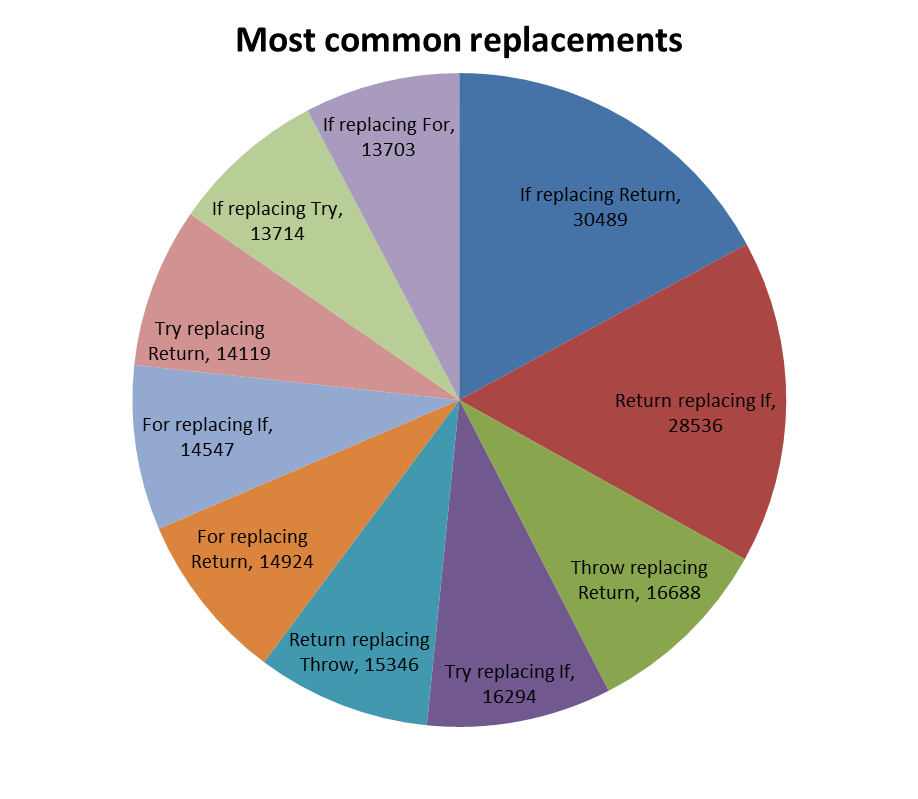
\includegraphics[scale=0.5]{g1.png}

\subsubsection{Least common replacements}
On the opposite side of the data, we can see that the least common replacement was an Assert statement replacing a Type Declaration statement. This was the only replacement to have zero appearances in our search through the 46,301,429 files being fixed. Close to it, as the second least common replacement was replacing a Do statement for a Type Declaration statement, with one appearance in our code database, and on third place, the replacement of a Label being replaced by a Type Declaration Statement had one appearance in our code database.

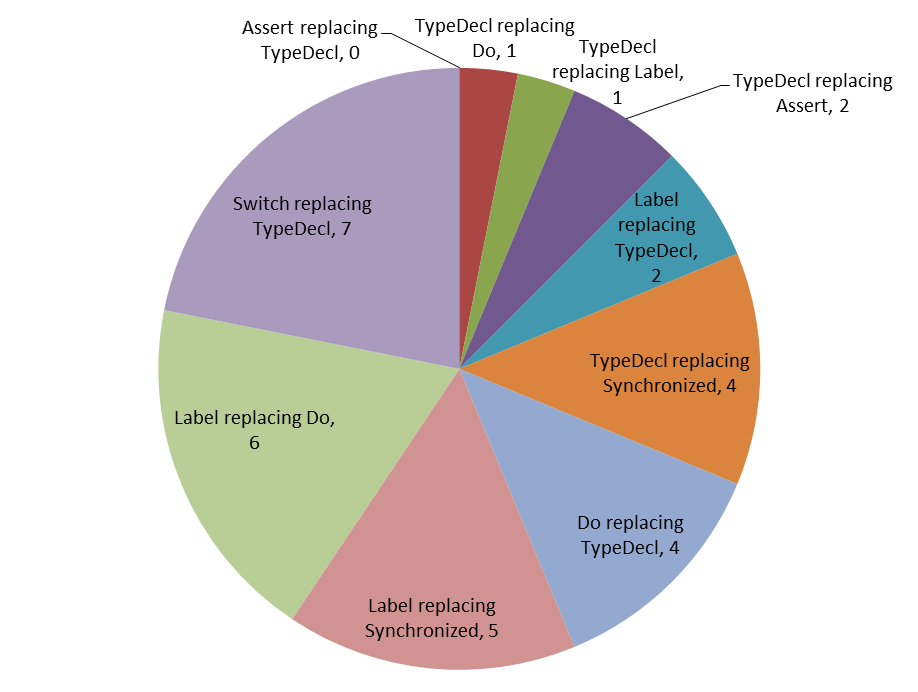
\includegraphics[scale=0.5]{g2.png}

\section{Related Work}
A similar study was performed by Dongsun Kim et al. \cite{dongsun} in which they look for the most common ways in which programmers patch bugs in software. The researchers developed a variation of the tool Genprog \cite{weimer}\cite{claire} with several different templates resembling patters programmers use to patch bugs. 

A good complement for this paper is \cite{hao}, where they search additions and deletions in a smaller data set. In this paper, we focus on the replacements, which have been left out of the analysis of \cite{hao}. 



\section{Conclusions}
The findings of our study provide a set of useful guidelines for automatic program repair tools with which their search for a patch can be now improved by having the knowledge of how likely it is to replace a faulty statement by the different kinds of statements available.


%\end{document}  % This is where a 'short' article might terminate


%
% The following two commands are all you need in the
% initial runs of your .tex file to
% produce the bibliography for the citations in your paper.
\bibliographystyle{abbrv}
\bibliography{sigproc}  % sigproc.bib is the name of the Bibliography in this case
% You must have a proper ".bib" file
%  and remember to run:
% latex bibtex latex latex
% to resolve all references
%
% ACM needs 'a single self-contained file'!
%
%APPENDICES are optional
%\balancecolumns


\begin{thebibliography}{9}

\bibitem{robert}
  Robert Dyer et al.,
  \emph{Boa: A Language and Infrastructure for Analyzing Ultra-Large-Scale Software Repositories},
35th International Conference on Software Engineering; ICSE 2013, San Francisco CA, USA

\bibitem{hao}
Hao Zhong, Zhendong Su
\emph{An Empirical Study on Real Bug Fixes},
In Proceedings of ICSE 2015, Firenze, Italy, May 16-24, 2015.

\bibitem{kai}
Kai Pan et al.
\emph{Towards an understanding of bug fix patterns},
Journal
Empirical Software Engineering
Volume 14 Issue 3, June 2009 
Pages 286 - 315 

\bibitem{dongsun}
Dongsun Kim et al.
\emph{Automatic patch generation learned from human-written patches},
Proceeding
ICSE '13 Proceedings of the 2013 International Conference on Software Engineering

\bibitem{zach}
Zachary P.Fry and Westley Weimer
\emph{A human study of fault localization accuracy},
ICSM '10 Proceedings of the 2010 IEEE International Conference on Software Maintenance

\bibitem{claire}
Claire Le Goues, ThanhVu Nguyen, Stephanie Forrest, Westley Weimer
\emph{GenProg: A Generic Method for Automated Software Repair.} 
IEEE Trans. Software Engineering 38(1): 54-72 (January/February 2012) 

\bibitem{weimer}
Westley Weimer, ThanVu Nguyen, Claire Le Goues, Stephanie Forrest
\emph{Automatically Finding Patches Using Genetic Programming.}
International Conference on Software Engineering (ICSE) 2009: 364-374

\end{thebibliography}

%\balancecolumns % GM June 2007
% That's all folks!
\end{document}
